La clase anterior concluyó la comparación entre la suspensión y el desplazamiento de espectros e introdujo varias construcciones nivel a nivel. Ahora completaremos esa discusión con el producto smash de dos espectros y explicaremos por qué su definición requiere signos. Después estudiaremos los $\Omega$-espectros: calcularemos sus grupos de homotopía, probaremos que una equivalencia estable entre ellos es una equivalencia nivel a nivel y construiremos explícitamente un reemplazo fibrante $X\to RX$. Finalmente introduciremos las celdas estables de un espectro celular y veremos que, con su estructura celular habitual, el espectro esfera tiene una única celda estable de dimensión cero.

Trabajaremos con aplicaciones y homotopías punteadas. Los morfismos estructurales se escribirán $\xi_n\colon X_n\wedge S^1\to X_{n+1}$ y sus adjuntos $\xi_n^{\perp}\colon X_n\to\Omega X_{n+1}$. Cuando intervengan dos espectros, distinguiremos sus morfismos mediante los superíndices $X$ e $Y$. Omitiremos las identificaciones asociativas del producto smash; al usar adjunciones indicaremos qué coordenada se evalúa, pues su orden será esencial.

%%%%%%%%%%%%%%%%%%%%%%%%%%%%%%%%%%%%%%%%%%%%%%%%%%%%%%%%%%%%%%%%%%%%%%%%%%%%%%%
\section{El producto smash de espectros}
%%%%%%%%%%%%%%%%%%%%%%%%%%%%%%%%%%%%%%%%%%%%%%%%%%%%%%%%%%%%%%%%%%%%%%%%%%%%%%%

% P1--P2.
\subsection{La construcción artesanal}

Sean $X$ e $Y$ espectros secuenciales. Fijemos una sucesión de parejas $(p_n,q_n)\in\mathbb N^2$ tal que $(p_0,q_0)=(0,0)$, en cada paso aumente exactamente uno de los índices en una unidad y ambos tiendan a infinito. Es decir, para cada $n$ se cumple una de las dos posibilidades
\[
(p_{n+1},q_{n+1})=(p_n+1,q_n)
\quad\text{o}\quad
(p_{n+1},q_{n+1})=(p_n,q_n+1),
\]
y $\lim_n p_n=\lim_n q_n=\infty$. En particular, $p_n+q_n=n$.

\begin{defi}\label{defi:c10-smash-artesanal}
El \emph{producto smash artesanal} de $X$ e $Y$, relativo a la sucesión elegida, tiene por niveles $(X\wedge Y)_n=X_{p_n}\wedge Y_{q_n}$. Si aumenta $q_n$, su morfismo estructural es
\[
\begin{tikzcd}[column sep=large]
X_{p_n}\wedge Y_{q_n}\wedge S^1
\arrow[r,"1\wedge\xi^Y_{q_n}"] & X_{p_n}\wedge Y_{q_n+1}.
\end{tikzcd}
\]
Si aumenta $p_n$, el morfismo estructural es la composición del siguiente triángulo:
\[
\begin{tikzcd}[column sep=large,row sep=large]
X_{p_n}\wedge Y_{q_n}\wedge S^1
\arrow[r,"1\wedge\tau_{q_n}"] \arrow[dr,swap,"\xi^{X\wedge Y}_n"]
& X_{p_n}\wedge S^1\wedge Y_{q_n}
\arrow[d,"\xi^X_{p_n}\wedge1"]\\
& X_{p_n+1}\wedge Y_{q_n}.
\end{tikzcd}
\]
Aquí $\tau_q\colon Y_q\wedge S^1\to S^1\wedge Y_q$ está dada por $\tau_q[y,z]=[z^{(-1)^q},y]$. Visto $S^1$ como el círculo unidad de $\mathbb C$, se tiene $z^{(-1)^q}=z$ si $q$ es par y $z^{(-1)^q}=\overline z$ si $q$ es impar.
\end{defi}

La elección de $(p_n,q_n)$ forma parte de esta definición. Se mencionó en clase el resultado de Adams según el cual distintas elecciones producen espectros establemente equivalentes; su demostración no se desarrollará aquí. El objetivo inmediato es entender el signo de la definición y comprobar que los grupos de homotopía no dependen del camino elegido.

% P3--P6. Malla de grupos, primer cuadrado y comparación de sus dos caminos.
\subsection{Por qué aparecen los signos}

La motivación es que $\pi_k(X\wedge Y)$ sea el colímite de una malla cuyos términos sean $\pi_{k+p+q}(X_p\wedge Y_q)$ y cuyas flechas procedan de los morfismos estructurales. El comienzo de la malla es
\[
\begin{tikzcd}[row sep=large]
\vdots & \vdots & \vdots\\
\pi_{k+2}(X_0\wedge Y_2) \arrow[u] \arrow[r]
& \pi_{k+3}(X_1\wedge Y_2) \arrow[u] \arrow[r]
& \pi_{k+4}(X_2\wedge Y_2) \arrow[u] \arrow[r] & \cdots\\
\pi_{k+1}(X_0\wedge Y_1) \arrow[u] \arrow[r]
& \pi_{k+2}(X_1\wedge Y_1) \arrow[u] \arrow[r]
& \pi_{k+3}(X_2\wedge Y_1) \arrow[u] \arrow[r] & \cdots\\
\pi_k(X_0\wedge Y_0) \arrow[u] \arrow[r]
& \pi_{k+1}(X_1\wedge Y_0) \arrow[u] \arrow[r]
& \pi_{k+2}(X_2\wedge Y_0) \arrow[u] \arrow[r] & \cdots
\end{tikzcd}
\]
Cada flecha consiste en suspender una clase y componer con el correspondiente morfismo estructural. Las verticales utilizan $1\wedge\xi^Y_q$ y las horizontales utilizan $(\xi^X_p\wedge1)\circ(1\wedge\tau_q)$. Para representar esta malla como un diagrama sobre el conjunto ordenado $\mathbb N^2$ necesitamos que todos sus cuadrados conmuten. Si $k<0$, se omiten los términos cuyo índice de homotopía aún no está definido; en cualquier caso podemos restringirnos a una región cofinal donde esos índices sean al menos dos.

Veamos qué ocurriría si usáramos la permutación ordinaria $\tau[y,z]=[z,y]$, sin conjugación. Escribamos $v_{p,q}=(1\wedge\xi_q^Y)_*\circ\Sigma$ y $u_{p,q}=((\xi_p^X\wedge1)\circ(1\wedge\tau))_*\circ\Sigma$ para las transiciones sin signo. El primer cuadrado sería
\[
\begin{tikzcd}[column sep=large,row sep=large]
\pi_{k+1}(X_0\wedge Y_1) \arrow[r,"u_{0,1}"]
& \pi_{k+2}(X_1\wedge Y_1)\\
\pi_k(X_0\wedge Y_0) \arrow[u,"v_{0,0}"] \arrow[r,"u_{0,0}"']
& \pi_{k+1}(X_1\wedge Y_0) \arrow[u,"v_{1,0}"'].
\end{tikzcd}
\]
Este cuadrado no conmuta en general. Para ver la diferencia, tomemos una clase representada por $g\colon S^k\to X_0\wedge Y_0$; en este primer cuadrado suponemos $k\ge0$, y para los demás grados hacemos la misma cuenta a partir de un término donde el grupo esté definido. El camino vertical seguido del horizontal daría la clase de
\[
(\xi^X_0\wedge1)\circ(1\wedge\tau)
\circ(1\wedge\xi^Y_0\wedge1)\circ(g\wedge1\wedge1),
\]
mientras que el camino horizontal seguido del vertical daría la clase de
\[
(1\wedge\xi^Y_0)\circ(\xi^X_0\wedge1\wedge1)
\circ(1\wedge\tau\wedge1)\circ(g\wedge1\wedge1).
\]
Ambas composiciones empiezan con $g\wedge1\wedge1$. Por tanto, basta comparar los dos caminos del siguiente diagrama, que \emph{no} conmuta en general:
\[
\begin{tikzcd}[column sep=3.2em,row sep=large]
X_0\wedge Y_0\wedge S^1\wedge S^1
\arrow[r,"1\wedge\xi^Y_0\wedge1"] \arrow[d,"1\wedge\tau\wedge1"']
& X_0\wedge Y_1\wedge S^1 \arrow[r,"1\wedge\tau"]
& X_0\wedge S^1\wedge Y_1 \arrow[d,"\xi^X_0\wedge1"]\\
X_0\wedge S^1\wedge Y_0\wedge S^1
\arrow[r,"\xi^X_0\wedge1\wedge1"']
& X_1\wedge Y_0\wedge S^1 \arrow[r,"1\wedge\xi^Y_0"']
& X_1\wedge Y_1.
\end{tikzcd}
\]
En efecto, el camino superior lleva $[x,y,z_1,z_2]$ sucesivamente a $[x,\xi^Y_0(y,z_1),z_2]$, a $[x,z_2,\xi^Y_0(y,z_1)]$ y finalmente a $[\xi^X_0(x,z_2),\xi^Y_0(y,z_1)]$. El inferior lo lleva a $[x,z_1,y,z_2]$, después a $[\xi^X_0(x,z_1),y,z_2]$ y finalmente a $[\xi^X_0(x,z_1),\xi^Y_0(y,z_2)]$. La diferencia es precisamente el intercambio de $z_1$ y $z_2$.

Así, los dos caminos se vuelven iguales si precomponemos uno de ellos con
\[
1\wedge1\wedge\tau\colon
X_0\wedge Y_0\wedge S^1\wedge S^1
\longrightarrow X_0\wedge Y_0\wedge S^1\wedge S^1.
\]
Pero la transposición $\tau\colon S^1\wedge S^1\to S^1\wedge S^1$ tiene grado $-1$. Para compensarla, cambiamos la flecha $X_0\wedge Y_1\wedge S^1\to X_0\wedge S^1\wedge Y_1$ por la aplicación $[x,y,z]\mapsto[x,\overline z,y]$. Este cambio afecta solo al camino superior y aporta otro grado $-1$. La composición de ambos cambios en $S^1\wedge S^1\cong S^2$ tiene grado $1$ y, por tanto, es homotópica a la identidad mediante una homotopía punteada. El cuadrado resultante sí conmuta al pasar a grupos de homotopía.

La misma corrección debe alternarse de una fila a la siguiente. En el cuadrado que parte de $(p,q)$, los valores finales de los caminos superior e inferior son, respectivamente,
\[
[\xi^X_p(x,z_2^{(-1)^{q+1}}),\xi^Y_q(y,z_1)]
\quad\text{y}\quad
[\xi^X_p(x,z_1^{(-1)^q}),\xi^Y_q(y,z_2)].
\] Precomponer este último con la aplicación de las dos coordenadas circulares $[z_1,z_2]\mapsto[\overline z_2,z_1]$ produce exactamente el primero. Esta aplicación vuelve a tener grado $1$. Por ello todos los cuadrados conmutan salvo homotopía antes de tomar grupos de homotopía y conmutan estrictamente después de tomarlos. Esto explica el factor $(-1)^q$ de la definición.

% P7.
\subsection{Cofinalidad y el espectro esfera}

La sucesión $(p_n,q_n)$ determina un camino cofinal en la malla: dada cualquier pareja $(p,q)$, existe $n$ tal que $p\le p_n$ y $q\le q_n$, pues ambos índices tienden a infinito. Como $p_n+q_n=n$, obtenemos
\[
\operatorname*{colim}_{(p,q)\in\mathbb N^2}
\pi_{k+p+q}(X_p\wedge Y_q)
\cong \operatorname*{colim}_n\pi_{k+n}(X_{p_n}\wedge Y_{q_n})
=\pi_k(X\wedge Y).
\]
Por tanto, todas las elecciones del camino dan los mismos grupos de homotopía. Esto no demuestra por sí solo la equivalencia estable entre las construcciones: todavía haría falta un morfismo, o un zigzag de morfismos, que indujera los isomorfismos. Esa es la parte adicional del resultado de Adams mencionado antes.

\begin{ejer}\label{ejer:c10-unidad-smash}
Sea $\mathbb S$ el espectro esfera. Probar que $Y\wedge\mathbb S\simeq_s Y$. Como pista, elegir una sucesión $(p_n,q_n)$ conveniente y utilizar las composiciones de los morfismos estructurales $Y_p\wedge S^q\to Y_{p+q}$, teniendo en cuenta los signos del producto smash.
\end{ejer}
\begin{sol}
Identificamos $S^q=(S^1)^{\wedge q}$ y escribimos $\sigma_{p,q}\colon Y_p\wedge S^q\to Y_{p+q}$ para la composición de $q$ morfismos estructurales, con $\sigma_{p,0}=1$. Fijado un camino admisible, pongamos $Z=Y\wedge\mathbb S$ y definamos $a_n=\sigma_{p_n,q_n}\colon Z_n\to Y_n$.

\emph{Estas aplicaciones forman un morfismo débil.} Si aumenta $q_n$, el cuadrado estructural conmuta estrictamente, pues $\sigma_{p,q+1}=\xi_{p+q}^Y\circ(\sigma_{p,q}\wedge1)$. Si aumenta $p_n$, los dos caminos son $\sigma_{p,q+1}$ y $\sigma_{p,q+1}\circ(1\wedge\beta_q)$, donde
\[
\beta_q[z_1,\ldots,z_q,t]
=[t^{(-1)^q},z_1,\ldots,z_q].
\]
La permutación cíclica tiene grado $(-1)^q$ y la posible conjugación aporta otro factor $(-1)^q$. Por tanto, $\beta_q$ tiene grado $1$ y es homotópica a la identidad; para $q=0$ es la identidad. Así, los cuadrados conmutan hasta homotopía punteada. Por el resultado sobre morfismos débiles de la clase anterior, obtenemos un zigzag $Z\xleftarrow{r}C\xrightarrow{a'}Y$, con $r$ una equivalencia nivel a nivel y $a'_n\simeq a_n\circ r_n$.

\emph{El morfismo inducido en homotopía estable es un isomorfismo.} Fijemos $k\in\mathbb Z$ y consideremos $A_{p,q}=\pi_{k+p+q}(Y_p\wedge S^q)$, restringiéndonos, si hace falta, a $p\ge\max\{0,2-k\}$. Sean $H_{p,q}$ y $V_{p,q}$ las transiciones horizontal y vertical de la malla con signos; aquí $V_{p,q}$ es simplemente la suspensión. Hay además diagonales
\[
D_{p,q+1}=(\xi_p^Y\wedge1_{S^q})_*\colon
A_{p,q+1}\longrightarrow A_{p+1,q}.
\]
Estas dividen cada cuadrado en dos triángulos conmutativos:
\[
\begin{tikzcd}[column sep=large,row sep=large]
A_{p,q+1} \arrow[r,"H_{p,q+1}"] \arrow[dr,"D_{p,q+1}" description]
& A_{p+1,q+1}\\
A_{p,q} \arrow[u,"V_{p,q}"] \arrow[r,"H_{p,q}"']
& A_{p+1,q} \arrow[u,"V_{p+1,q}"'].
\end{tikzcd}
\]
En efecto, $D_{p,q+1}V_{p,q}=H_{p,q}$ porque las aplicaciones que las inducen difieren por $1\wedge\beta_q\simeq1$; de igual manera, $V_{p+1,q}D_{p,q+1}=H_{p,q+1}$ usando $\beta_{q+1}\simeq1$. Estas identidades también hacen compatibles las diagonales con las transiciones horizontales. Al tomar colímites en $p$, las verticales y las diagonales inducen aplicaciones inversas: sus composiciones son transiciones horizontales, que representan la identidad en el colímite. Por ello todos los colímites de las filas se identifican con el de la fila $q=0$, que es $\pi_k(Y)$, y
\[
\pi_k(Z)\cong\operatorname*{colim}_{q}\operatorname*{colim}_{p}A_{p,q}
\cong\operatorname*{colim}_{p}A_{p,0}=\pi_k(Y).
\]
El primer isomorfismo es el de cofinalidad probado antes. El segundo está inducido por aplicar sucesivamente las diagonales; sobre $A_{p,q}$, su composición es precisamente $(\sigma_{p,q})_*$. Por tanto, el isomorfismo obtenido es el inducido por $(a_n)$. Como $a'_n\simeq a_n r_n$ y $r$ es una equivalencia estable, $a'$ también induce isomorfismos en todos los grupos estables. El zigzag anterior demuestra $Y\wedge\mathbb S\simeq_sY$.
\end{sol}

El ejercicio expresa el papel del espectro esfera como unidad por la derecha del producto smash en la categoría homotópica estable. El profesor mencionó también que $\mathbb S\wedge Y\simeq_sY$, aunque precisó que el ejercicio propuesto era el anterior. No se trata de una igualdad nivel a nivel: en general, un nivel de $Y\wedge\mathbb S$ tiene la forma $Y_{p_n}\wedge S^{q_n}$, que no coincide con $Y_n$. La estructura monoidal simétrica completa se estudiará más adelante.

%%%%%%%%%%%%%%%%%%%%%%%%%%%%%%%%%%%%%%%%%%%%%%%%%%%%%%%%%%%%%%%%%%%%%%%%%%%%%%%
\section{Los \texorpdfstring{$\Omega$}{Omega}-espectros y el reemplazo fibrante}
%%%%%%%%%%%%%%%%%%%%%%%%%%%%%%%%%%%%%%%%%%%%%%%%%%%%%%%%%%%%%%%%%%%%%%%%%%%%%%%

% P8--P9.
\subsection{Grupos de homotopía y espacios de lazos infinitos}

Recordemos que $X$ es un \emph{$\Omega$-espectro} si cada adjunto $\xi_n^{\perp}\colon X_n\to\Omega X_{n+1}$ es una equivalencia débil. En ese caso se simplifica el cálculo de los grupos de homotopía estable: las transiciones del sistema que define $\pi_k(X)$ se pueden escribir como
\[
\pi_{k+n}(X_n)
\xrightarrow{(\xi_n^{\perp})_*}
\pi_{k+n}(\Omega X_{n+1})
\xrightarrow[\cong]{\operatorname{adj}}
\pi_{k+n+1}(X_{n+1}).
\]
El primer morfismo es un isomorfismo porque $\xi_n^{\perp}$ es una equivalencia débil y el segundo lo es por adjunción. Por tanto, el colímite se identifica con cualquiera de sus términos: $\pi_k(X)\cong\pi_{k+n}(X_n)$ siempre que $n\ge0$ y $k+n\ge0$. Para índice cero obtenemos primero una biyección de componentes; las identificaciones con espacios de lazos le dan la estructura de grupo.

En particular, $\pi_k(X)\cong\pi_k(X_0)$ para $k\ge0$, mientras que para $k\le0$ podemos escribir $\pi_k(X)\cong\pi_0(X_{-k})$. La expresión uniforme es $\pi_k(X)\cong\pi_{n_0}(X_{n_0-k})$, con $n_0\ge\max\{k,0\}$. No se utiliza el nivel $X_{-k}$ cuando $-k<0$ en un espectro indexado por $\mathbb N$.

Las equivalencias estructurales proporcionan además una sucesión
\[
X_0\xrightarrow{\simeq_w}\Omega X_1
\xrightarrow{\simeq_w}\Omega^2X_2
\xrightarrow{\simeq_w}\cdots
\xrightarrow{\simeq_w}\Omega^rX_r\xrightarrow{\simeq_w}\cdots.
\]
Así, $X_0$ admite desuspensiones iteradas compatibles y es un \emph{espacio de lazos infinitos}. Para un $\Omega$-espectro escribimos $\Omega^\infty X=X_0$. Esta descripción permite construir teorías de cohomología a partir de métodos de reconocimiento y construcciones combinatorias de espacios de lazos infinitos, tema al que se volverá más adelante.

\begin{nota}
La estructura de espacio de lazos infinitos incluye la compatibilidad de las desuspensiones; no consiste únicamente en un espacio topológico. Además, $X_0$ detecta los grupos estables de grados no negativos, pero no los negativos. La equivalencia habitual entre espacios de lazos infinitos y espectros se formula para espectros conectivos, es decir, aquellos con $\pi_k=0$ para $k<0$.
\end{nota}

% P9--P10. Se corrigen la orientación y los índices del segundo cuadrado.
\subsection{Equivalencias estables entre \texorpdfstring{$\Omega$}{Omega}-espectros}

\begin{prop}\label{prop:c10-omega-equivalencias}
Una equivalencia estable entre $\Omega$-espectros es una equivalencia nivel a nivel. En consecuencia, para un morfismo entre $\Omega$-espectros ambas condiciones son equivalentes.
\end{prop}
\begin{proof}
Sea $f\colon X\to Y$ una equivalencia estable. Para todo $n\ge0$ y $k\ge1$ tenemos el cuadrado conmutativo
\[
\begin{tikzcd}[column sep=large,row sep=large]
\pi_k(X_n) \arrow[r,"(f_n)_*"] \arrow[d,"\cong"']
& \pi_k(Y_n) \arrow[d,"\cong"]\\
\pi_{k-n}(X) \arrow[r,"f_*"',"\cong"]
& \pi_{k-n}(Y).
\end{tikzcd}
\]
Las verticales son los isomorfismos calculados antes y la horizontal inferior es un isomorfismo por hipótesis. Por ello $(f_n)_*$ también es un isomorfismo.

Esto prueba que $f_n$ restringe a una equivalencia débil entre las componentes del punto base. Para concluir que es una equivalencia débil de todo el espacio hay que considerar las demás componentes. Aplicamos lo anterior en el nivel $n+1$: todo lazo basado en $X_{n+1}$ permanece en su componente del punto base, y lo mismo ocurre en $Y_{n+1}$. Así, $\Omega f_{n+1}$ es una equivalencia débil. En detalle, induce una biyección en componentes porque estas son los elementos de $\pi_1$, y los grupos de homotopía en cualquier componente se trasladan a los de la componente del lazo constante mediante concatenación con un lazo y su inverso.

La condición de que $f$ sea un morfismo de espectros, escrita mediante adjuntos, da el siguiente cuadrado, con los índices y la orientación correspondientes a $\xi_n^\perp\colon X_n\to\Omega X_{n+1}$:
\[
\begin{tikzcd}[column sep=large,row sep=large]
X_n \arrow[r,"f_n"] \arrow[d,"\xi_n^{X,\perp}"',"\simeq_w"]
& Y_n \arrow[d,"\xi_n^{Y,\perp}","\simeq_w"']\\
\Omega X_{n+1} \arrow[r,"\Omega f_{n+1}"',"\simeq_w"]
& \Omega Y_{n+1}.
\end{tikzcd}
\]
Las verticales son equivalencias débiles porque $X$ e $Y$ son $\Omega$-espectros. Por la propiedad de dos de tres, $f_n$ también es una equivalencia débil. Esto vale para todo $n\ge0$, incluido $n=0$. El recíproco, que una equivalencia nivel a nivel induce isomorfismos en los colímites que definen los grupos estables, vale para cualesquiera espectros.
\end{proof}

% P10--P11.
\subsection{Construcción del reemplazo mediante telescopios}

Dado un espectro secuencial $X$, definimos
\[
(RX)_n=\operatorname*{hocolim}_{m\ge0}
\bigl(X_n\xrightarrow{\xi_n^{\perp}}\Omega X_{n+1}
\xrightarrow{\Omega\xi_{n+1}^{\perp}}\Omega^2X_{n+2}
\xrightarrow{\Omega^2\xi_{n+2}^{\perp}}\cdots\bigr).
\]
Este colímite homotópico es el telescopio punteado de la sucesión. Se forma con los cilindros $(\Omega^mX_{n+m})\wedge I_+$, pegando el extremo $s=1$ del cilindro $m$ al extremo $s=0$ del siguiente por $\Omega^m\xi_{n+m}^{\perp}$. Para $a\in\Omega^mX_{n+m}$, la pegadura es
\[
[a,1]=[\Omega^m\xi_{n+m}^{\perp}(a),0],
\]
y todos los segmentos de los puntos base quedan colapsados al punto base. El cilindro al que pertenece $a$ se sobreentiende en la notación $[a,s]$.

\begin{center}
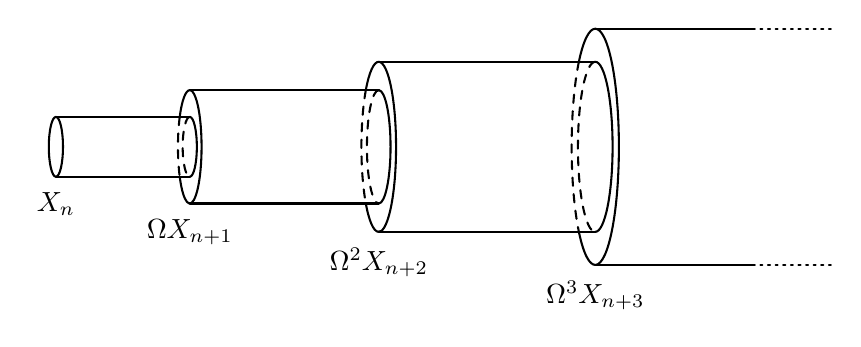
\begin{tikzpicture}[x=1cm,y=1cm,line width=.75pt,
                    line cap=round,line join=round]
  % Tapa izquierda completamente visible.
  \def\tapaVisible#1#2#3{%
    \draw (#1,0) ellipse [x radius=#2,y radius=#3];%
  }

  % Tapa derecha: mitad izquierda oculta.
  \def\tapaDerecha#1#2#3{%
    \draw[dashed] (#1,#3)
      arc[start angle=90,end angle=270,
          x radius=#2,y radius=#3];
    \draw (#1,#3)
      arc[start angle=90,end angle=-90,
          x radius=#2,y radius=#3];%
  }

  % Tapa izquierda: arco oculto por el cilindro anterior.
  \def\tapaIzquierda#1#2#3#4{%
    \pgfmathsetmacro{\anguloOculto}{asin(#4/#3)}%
    \draw (#1,#3)
      arc[start angle=90,end angle={180-\anguloOculto},
          x radius=#2,y radius=#3];
    \draw[dashed] ({#1-#2*cos(\anguloOculto)},#4)
      arc[start angle={180-\anguloOculto},
          end angle={180+\anguloOculto},
          x radius=#2,y radius=#3];
    \draw ({#1-#2*cos(\anguloOculto)},{-#4})
      arc[start angle={180+\anguloOculto},end angle=450,
          x radius=#2,y radius=#3];%
  }

  % Primer cilindro.
  \draw (2.55,.38) -- (4.25,.38)
        (2.55,-.38) -- (4.25,-.38);
  \tapaVisible{2.55}{.09}{.38}
  \tapaDerecha{4.25}{.09}{.38}
  \node[below=2pt] at (2.55,-.38) {$X_n$};

  % Segundo cilindro.
  \draw (4.25,.72) -- (6.65,.72)
        (4.25,-.72) -- (6.65,-.72);
  \tapaIzquierda{4.25}{.15}{.72}{.38}
  \tapaDerecha{6.65}{.15}{.72}
  \node[below=2pt] at (4.25,-.72) {$\Omega X_{n+1}$};

  % Tercer cilindro.
  \draw (6.65,1.08) -- (9.40,1.08)
        (6.65,-1.08) -- (9.40,-1.08);
  \tapaIzquierda{6.65}{.22}{1.08}{.72}
  \tapaDerecha{9.40}{.22}{1.08}
  \node[below=2pt] at (6.65,-1.08) {$\Omega^2 X_{n+2}$};

  % Último cilindro: continuación indefinida, sin tapa derecha.
  \tapaIzquierda{9.40}{.30}{1.50}{1.08}
  \draw (9.40,1.50) -- (11.40,1.50)
        (9.40,-1.50) -- (11.40,-1.50);
  \draw[dotted] (11.40,1.50) -- (12.40,1.50)
                (11.40,-1.50) -- (12.40,-1.50);
  \node[below=2pt] at (9.40,-1.50) {$\Omega^3 X_{n+3}$};
\end{tikzpicture}
\end{center}

Para fijar el orden de las coordenadas, identificamos $\Omega^m Z$ con las aplicaciones punteadas $(S^1)^{\wedge m}\to Z$. En $\Omega^m\xi_j^{\perp}$, la coordenada de lazo nueva se coloca a la derecha: para $a\in\Omega^mX_j$,
\[
\bigl(\Omega^m\xi_j^{\perp}(a)\bigr)(u_1,\ldots,u_m,v)
=\xi_j\bigl(a(u_1,\ldots,u_m),v\bigr).
\]
Por otra parte, al identificar $\Omega^{m+1}Z$ con $\Omega(\Omega^mZ)$, la coordenada exterior es la primera. Esta distinción es la que permite que las adjunciones utilizadas más adelante sean compatibles.

Comparemos ahora la sucesión anterior con la que resulta al omitir su primer término:
\[
\begin{tikzcd}[column sep=large,row sep=large]
X_n \arrow[r,"\xi_n^{\perp}"] \arrow[d,"\xi_n^{\perp}"']
& \Omega X_{n+1} \arrow[r,"\Omega\xi_{n+1}^{\perp}"] \arrow[d,"\Omega\xi_{n+1}^{\perp}"']
& \Omega^2X_{n+2} \arrow[r] \arrow[d,"\Omega^2\xi_{n+2}^{\perp}"] & \cdots\\
\Omega X_{n+1} \arrow[r,"\Omega\xi_{n+1}^{\perp}"']
& \Omega^2X_{n+2} \arrow[r,"\Omega^2\xi_{n+2}^{\perp}"']
& \Omega^3X_{n+3} \arrow[r] & \cdots.
\end{tikzcd}
\]
Los cuadrados conmutan estrictamente, pues sus dos composiciones son las mismas aplicaciones sucesivas. Al tomar telescopios obtenemos
\[
g_n\colon(RX)_n\longrightarrow
\operatorname*{hocolim}_{m\ge0}\Omega^{m+1}X_{n+m+1}.
\]
Su fórmula es $g_n[a,s]=[\Omega^m\xi_{n+m}^{\perp}(a),s]$ para $a\in\Omega^mX_{n+m}$; a la derecha, el elemento pertenece al cilindro $m$ de la sucesión que empieza con $\Omega X_{n+1}$.

Existe asimismo una aplicación natural que saca un lazo del telescopio:
\[
\lambda_n\colon
\operatorname*{hocolim}_{m\ge0}\Omega^{m+1}X_{n+m+1}
\longrightarrow\Omega(RX)_{n+1},
\qquad
\lambda_n[a,s](t)=[a(t),s].
\]
Aquí $a$ se considera un lazo con valores en $\Omega^mX_{n+m+1}$. La fórmula respeta las pegaduras porque evaluar la coordenada exterior conmuta con las aplicaciones del sistema.

La aplicación $\lambda_n$ es una equivalencia débil. Se utiliza aquí la propiedad del telescopio de que sus grupos de homotopía son los colímites de los grupos de los términos: las aplicaciones desde esferas y las homotopías se pueden representar, salvo homotopía, en una etapa finita. Aplicando además la adjunción suspensión--lazos, obtenemos, para $i\ge0$,
\[
\begin{aligned}
\pi_i\!\left(\operatorname*{hocolim}_m\Omega^{m+1}X_{n+m+1}\right)
&\cong\operatorname*{colim}_m\pi_{i+1}(\Omega^mX_{n+m+1})\\
&\cong\pi_{i+1}((RX)_{n+1})
\cong\pi_i(\Omega(RX)_{n+1}).
\end{aligned}
\]
Estos isomorfismos están inducidos por $\lambda_n$. El mismo argumento para familias de lazos basadas en un lazo cualquiera da los isomorfismos en las demás componentes; por tanto, no se trata solo de una comprobación en el lazo constante.

Definimos los adjuntos de los morfismos estructurales de $RX$ por la composición del triángulo
\[
\begin{tikzcd}[column sep=large,row sep=large]
(RX)_n \arrow[r,"g_n"] \arrow[dr,"(\xi'_n)^{\perp}"']
& \smash[b]{\operatorname*{hocolim}_{m\ge0}}\Omega^{m+1}X_{n+m+1}
\arrow[d,"\lambda_n", "\simeq_w"']\\
& \Omega(RX)_{n+1}.
\end{tikzcd}
\]
Por adjunción, esto define aplicaciones $\xi'_n\colon(RX)_n\wedge S^1\to(RX)_{n+1}$ y, con ellas, un espectro $RX$.

% P12--P14.
\subsection{Por qué el reemplazo es un \texorpdfstring{$\Omega$}{Omega}-espectro}

Probemos que $g_n$ es una equivalencia homotópica. Siguiendo la construcción de clase, consideremos la homotopía
\[
H\colon(RX)_n\times I\longrightarrow
\operatorname*{hocolim}_{m\ge0}\Omega^{m+1}X_{n+m+1}
\]
definida por
\[
H([a,s],t)=
\begin{cases}
[\xi_n^{\perp}(a),st],&a\in X_n,\\[2pt]
[a,s+t],&a\in\Omega^mX_{n+m},\ m\ge1,\ 0\le s\le1-t,\\[2pt]
[\Omega^m\xi_{n+m}^{\perp}(a),s-(1-t)],
&a\in\Omega^mX_{n+m},\ m\ge1,\ 1-t\le s\le1.
\end{cases}
\]
% En el segundo caso se usa el cilindro de $\Omega^mX_{n+m}$ en el telescopio de llegada y en el tercero se pasa al siguiente. 
Geométricamente, el primer cilindro se aplasta sobre el comienzo del telescopio de llegada, mientras que los demás se desplazan, repartiendo cada cilindro entre dos cilindros consecutivos.

\begin{center}
% Para fijar otra posición de la homotopía, cambie \tHom (0<tHom<1).
\begin{tikzpicture}[x=1cm,y=1cm,line width=.75pt,
                    line cap=round,line join=round,>=stealth]
  \def\L{2.2}       % Longitud común de los cilindros.
  \def\separacion{5}
  \def\tHom{.38}    % Valor de t representado.
  \def\alturaImagen{.40} % Distancia sobre el cilindro más ancho.

  \def\tapaVisible#1#2#3{%
    \draw (#1,0) ellipse [x radius=#2,y radius=#3];%
  }
  \def\tapaDerecha#1#2#3{%
    \draw[dashed] (#1,#3)
      arc[start angle=90,end angle=270,
          x radius=#2,y radius=#3];
    \draw (#1,#3)
      arc[start angle=90,end angle=-90,
          x radius=#2,y radius=#3];%
  }
  \def\tapaIzquierda#1#2#3#4{%
    \pgfmathsetmacro{\anguloOculto}{asin(#4/#3)}%
    \draw (#1,#3)
      arc[start angle=90,end angle={180-\anguloOculto},
          x radius=#2,y radius=#3];
    \draw[dashed] ({#1-#2*cos(\anguloOculto)},#4)
      arc[start angle={180-\anguloOculto},
          end angle={180+\anguloOculto},
          x radius=#2,y radius=#3];
    \draw ({#1-#2*cos(\anguloOculto)},{-#4})
      arc[start angle={180+\anguloOculto},end angle=450,
          x radius=#2,y radius=#3];%
  }
  \def\cuerpo#1#2{%
    \draw ({#1*\L},#2) -- ({(#1+1)*\L},#2)
          ({#1*\L},{-#2}) -- ({(#1+1)*\L},{-#2});%
  }
  \def\cuerpoAbierto#1#2{%
    \draw ({#1*\L},#2) -- ({(#1+.85)*\L},#2)
          ({#1*\L},{-#2}) -- ({(#1+.85)*\L},{-#2});
    \draw[dotted]
          ({(#1+.85)*\L},#2) -- ({(#1+1.2)*\L},#2)
          ({(#1+.85)*\L},{-#2}) -- ({(#1+1.2)*\L},{-#2});%
  }

  % Telescopio superior: X_n, Omega X_{n+1}, ...
  \cuerpo{0}{.38}
  \tapaVisible{0}{.09}{.38}
  \tapaDerecha{\L}{.09}{.38}
  \node[above=2pt] at (0,.38) {$X_n$};

  \cuerpo{1}{.72}
  \tapaIzquierda{\L}{.15}{.72}{.38}
  \tapaDerecha{2*\L}{.15}{.72}
  \node[above=2pt] at (\L,.72) {$\Omega X_{n+1}$};

  \cuerpo{2}{1.08}
  \tapaIzquierda{2*\L}{.22}{1.08}{.72}
  \tapaDerecha{3*\L}{.22}{1.08}
  \node[above=2pt] at ({2*\L},1.08) {$\Omega^2X_{n+2}$};

  \cuerpoAbierto{3}{1.50}
  \tapaIzquierda{3*\L}{.30}{1.50}{1.08}
  \node[above=2pt] at ({3*\L},1.50) {$\Omega^3X_{n+3}$};

  % Telescopio inferior: se omite X_n y se añade Omega^4 X_{n+4}.
  \begin{scope}[yshift=-\separacion cm]
    \cuerpo{0}{.72}
    \tapaVisible{0}{.15}{.72}
    \tapaDerecha{\L}{.15}{.72}
    \node[below=2pt] at (0,-.72) {$\Omega X_{n+1}$};

    \cuerpo{1}{1.08}
    \tapaIzquierda{\L}{.22}{1.08}{.72}
    \tapaDerecha{2*\L}{.22}{1.08}
    \node[below=2pt] at (\L,-1.08) {$\Omega^2X_{n+2}$};

    \cuerpo{2}{1.50}
    \tapaIzquierda{2*\L}{.30}{1.50}{1.08}
    \tapaDerecha{3*\L}{.30}{1.50}
    \node[below=2pt] at ({2*\L},-1.50) {$\Omega^3X_{n+3}$};

    \cuerpoAbierto{3}{1.86}
    \tapaIzquierda{3*\L}{.37}{1.86}{1.50}
    \node[below=2pt] at ({3*\L},-1.86) {$\Omega^4X_{n+4}$};

    % Segmentos de llegada por encima del cilindro más ancho
    % que interviene en cada imagen: forman una escalerita.
    % El primero representa [0,t] del primer cilindro inferior.
    \draw[rojoCIMAT,very thick]
      (0,{.72+\alturaImagen})
      -- ({\tHom*\L},{.72+\alturaImagen});
    \foreach \x in {0,\tHom}{
      \draw[rojoCIMAT] ({\x*\L},{.72+\alturaImagen-.08})
              -- ({\x*\L},{.72+\alturaImagen+.08});
    }
    \node[rojoCIMAT,below=-1.5pt,font=\scriptsize]
      at ({\tHom*\L},{.72+\alturaImagen-.08}) {$t$};

    % Los demás atraviesan una pegadura:
    % [t,1] del cilindro anterior unido a [0,t] del siguiente.
    \foreach \m/\radio in {1/1.08,2/1.50,3/1.86}{
      \pgfmathsetmacro{\ySegmento}{\radio+\alturaImagen}
      \draw[rojoCIMAT,very thick]
        ({(\m-1+\tHom)*\L},\ySegmento)
        -- ({(\m+\tHom)*\L},\ySegmento);
      \foreach \extremo in {0,1}{
        \draw[rojoCIMAT]
          ({(\m-1+\tHom+\extremo)*\L},{\ySegmento-.08})
          -- ({(\m-1+\tHom+\extremo)*\L},{\ySegmento+.08});
      }
      \node[rojoCIMAT,below=-1.5pt,font=\scriptsize]
        at ({(\m+\tHom)*\L},{\ySegmento-.08}) {$t$};
    }
  \end{scope}

  % Una flecha por cilindro superior; cada flecha termina
  % exactamente sobre su segmento rojo de llegada.
  \foreach \m/\radioSuperior/\radioInferior in
    {0/.38/.72,1/.72/1.08,2/1.08/1.50,3/1.50/1.86}{
    \pgfmathsetmacro{\xImagen}
      {(\m==0 ? .5*\tHom : \m-.5+\tHom)*\L}
    \pgfmathsetmacro{\yImagen}
      {-\separacion+\radioInferior+\alturaImagen}
    \pgfmathsetmacro{\yControl}{(-\radioSuperior+\yImagen)/2}
    \draw[rojoCIMAT,thick,->]
      ({(\m+.5)*\L},{-\radioSuperior})
      .. controls ({(\m+.5)*\L},\yControl)
               and (\xImagen,\yControl)
      .. (\xImagen,\yImagen);
  }
  \node[rojoCIMAT] at (8.65,-2.35) {$H_t$};
\end{tikzpicture}
\end{center}

Comprobemos que las fórmulas se pegan. En el punto $s=1-t$ del cilindro $m\ge1$, la segunda da $[a,1]$ y la tercera da $[\Omega^m\xi_{n+m}^{\perp}(a),0]$; son el mismo punto por la relación del telescopio. Para la primera pegadura, si $a\in X_n$, tanto $H([a,1],t)$ como $H([\xi_n^{\perp}(a),0],t)$ son $[\xi_n^{\perp}(a),t]$. Para las demás pegaduras, si $a\in\Omega^mX_{n+m}$ con $m\ge1$, las imágenes de $[a,1]$ y $[\Omega^m\xi_{n+m}^{\perp}(a),0]$ son ambas $[\Omega^m\xi_{n+m}^{\perp}(a),t]$. Las fórmulas son continuas en cada pieza y preservan el punto base, por lo que definen una homotopía punteada.

Cuando $t=1$, cada cilindro pasa al siguiente mediante la aplicación estructural correspondiente, conservando $s$; por tanto, $H_1=g_n$. Cuando $t=0$, el primer cilindro se aplasta sobre $\Omega X_{n+1}$ y todos los restantes quedan fijos. Este último mapa es la retracción del primer cilindro de aplicación sobre su extremo de llegada, así que es una equivalencia homotópica. Por consiguiente, $g_n$ también lo es. Como $\lambda_n$ es una equivalencia débil, $(\xi'_n)^{\perp}=\lambda_n\circ g_n$ es una equivalencia débil para todo $n$. Luego $RX$ es un $\Omega$-espectro.

% P14--P15.
\subsection{La inclusión de \texorpdfstring{$X$}{X} en su reemplazo}

Definimos $h_n\colon X_n\to(RX)_n$ mediante $h_n(x)=[x,0]$, es decir, incluyendo $X_n$ en el comienzo del primer cilindro.

\begin{ejer}\label{ejer:c10-inclusion-reemplazo}
Comprobar que las aplicaciones $h_n$ forman un morfismo de espectros $h\colon X\to RX$.
\end{ejer}
\begin{sol}
Basta comprobar que conmuta el cuadrado de adjuntos
\[
\begin{tikzcd}[column sep=large,row sep=large]
X_n \arrow[r,"h_n"] \arrow[d,"\xi_n^{\perp}"']
& (RX)_n \arrow[d,"(\xi'_n)^{\perp}"]\\
\Omega X_{n+1} \arrow[r,"\Omega h_{n+1}"'] & \Omega(RX)_{n+1}.
\end{tikzcd}
\]
Al evaluar ambas composiciones en $x\in X_n$ y después en $t\in S^1$, se obtiene en los dos casos $[\xi_n^{\perp}(x)(t),0]$: $g_n$ aplica $\xi_n^\perp$ en el primer cilindro y $\lambda_n$ evalúa el lazo, mientras que $\Omega h_{n+1}$ incluye su valor en el comienzo del telescopio siguiente. Por adjunción también conmuta el cuadrado de los morfismos estructurales, de modo que $h$ es un morfismo de espectros.
\end{sol}

Falta demostrar que este morfismo induce los isomorfismos de homotopía estable.

% P16--P21.
\subsection{El doble sistema de grupos de homotopía}

Fijemos $k\in\mathbb Z$ y tomemos $n$ suficientemente grande para que $k+n\ge2$. Consideremos la malla
\[
\begin{tikzcd}[column sep=2.5em,row sep=large]
\pi_{k+n}(X_n)
\arrow[r,"(\xi_n^{\perp})_*"]
\arrow[d,"\operatorname{adj}\circ(\xi_n^{\perp})_*"']
& \pi_{k+n}(\Omega X_{n+1})
\arrow[r,"(\Omega\xi_{n+1}^{\perp})_*"] \arrow[d]
& \pi_{k+n}(\Omega^2X_{n+2}) \arrow[r] \arrow[d] & \cdots\\
\pi_{k+n+1}(X_{n+1}) \arrow[r,"(\xi_{n+1}^{\perp})_*"'] \arrow[d]
& \pi_{k+n+1}(\Omega X_{n+2}) \arrow[r] \arrow[d]
& \pi_{k+n+1}(\Omega^2X_{n+3}) \arrow[r] \arrow[d] & \cdots\\
\pi_{k+n+2}(X_{n+2}) \arrow[r] \arrow[d]
& \pi_{k+n+2}(\Omega X_{n+3}) \arrow[r] \arrow[d]
& \pi_{k+n+2}(\Omega^2X_{n+4}) \arrow[r] \arrow[d] & \cdots\\
\vdots & \vdots & \vdots
\end{tikzcd}
\]
En cada fila, el índice de homotopía permanece fijo y las aplicaciones son las inducidas por las transiciones del telescopio. En cada columna, primero se aplica la transición del telescopio y después se usa la adjunción para convertir la primera coordenada de lazo en una coordenada de la esfera del dominio. El cuadrado general es
\[
\begin{tikzcd}[column sep=4.5em,row sep=huge]
\pi_{k+n}(\Omega^mX_{n+m})
\arrow[r,"(\Omega^m\xi_{n+m}^{\perp})_*"]
\arrow[d,"\operatorname{adj}\circ(\Omega^m\xi_{n+m}^{\perp})_*"']
& \pi_{k+n}(\Omega^{m+1}X_{n+m+1})
\arrow[d,"\operatorname{adj}\circ(\Omega^{m+1}\xi_{n+m+1}^{\perp})_*"]\\
\pi_{k+n+1}(\Omega^mX_{n+m+1})
\arrow[r,"(\Omega^m\xi_{n+m+1}^{\perp})_*"']
& \pi_{k+n+1}(\Omega^{m+1}X_{n+m+2}).
\end{tikzcd}
\]
Para comprobar la conmutatividad, precisemos dónde se toma el adjunto. Sea $g\colon S^{k+n}\to\Omega^mX_{n+m}$. El camino superior seguido del derecho está representado por
\[
\Bigl((\Omega^{m+1}\xi_{n+m+1}^{\perp})
\circ(\Omega^m\xi_{n+m}^{\perp})\circ g\Bigr)^{\perp},
\]
y el camino izquierdo seguido del inferior está representado por
\[
(\Omega^m\xi_{n+m+1}^{\perp})
\circ\Bigl((\Omega^m\xi_{n+m}^{\perp})\circ g\Bigr)^{\perp}.
\]
En estas dos fórmulas el símbolo ${}^{\perp}$ pasa de una aplicación hacia un espacio de lazos a una aplicación desde la suspensión. Para escribir las evaluaciones de forma legible, pongamos únicamente durante esta comprobación $b=(\Omega^m\xi_{n+m}^{\perp})\circ g$ y $F=\Omega^m\xi_{n+m+1}^{\perp}$. Las dos aplicaciones son $(\Omega F\circ b)^{\perp}$ y $F\circ b^{\perp}$, respectivamente. Evaluándolas en $[x,t]\in S^{k+n}\wedge S^1$, resulta
\[
\begin{aligned}
(\Omega F\circ b)^{\perp}[x,t]
&=(\Omega F)(b(x))(t)\\
&=F\bigl(b(x)(t)\bigr)
=F\bigl(b^{\perp}[x,t]\bigr).
\end{aligned}
\]
La igualdad es la naturalidad de la adjunción, pero podemos verificarla también en las coordenadas restantes, como en clase. Si $m\ge1$, ambos valores, evaluados en $(u_1,\ldots,u_{m+1})$, son
\[
\xi_{n+m+1}\!\left(
\xi_{n+m}\bigl(g(x)(t,u_1,\ldots,u_{m-1}),u_m\bigr),
u_{m+1}\right).
\]
Para $m=0$, ambos son $\xi_{n+1}(\xi_n(g(x),t),u_1)$. Así, los caminos coinciden como aplicaciones, y el cuadrado conmuta. La variable $t$ pasa a ser la primera coordenada de lazo al evaluar $b(x)$; intercambiarla con otra coordenada modificaría el argumento.

% P21--P24.
\subsection{Paso a colímites y equivalencia estable}

Por la descripción de los grupos de homotopía del telescopio y la conmutatividad anterior,
\[
\begin{aligned}
\pi_k(RX)
&=\operatorname*{colim}_n\pi_{k+n}((RX)_n)\\
&\cong\operatorname*{colim}_n\operatorname*{colim}_m
\pi_{k+n}(\Omega^mX_{n+m})\\
&\cong\operatorname*{colim}_m\operatorname*{colim}_n
\pi_{k+n}(\Omega^mX_{n+m}).
\end{aligned}
\]
La primera identificación está inducida por las inclusiones de las etapas en el telescopio. La segunda cambia el orden de los colímites: ambos colímites iterados son el colímite del mismo diagrama sobre las parejas $(n,m)$. No se cambian los elementos ni las aplicaciones del sistema.

Ahora tomaremos primero los colímites verticales. La primera columna ya da $\pi_k(X)$; probaremos que las flechas horizontales inducen isomorfismos entre los colímites de cualesquiera dos columnas consecutivas. Para ello añadimos al cuadrado general la diagonal de adjunción:
\[
\begin{tikzcd}[column sep=4.5em,row sep=huge]
\pi_{k+n}(\Omega^mX_{n+m})
\arrow[r,"(\Omega^m\xi_{n+m}^{\perp})_*"]
\arrow[d,"\operatorname{adj}\circ(\Omega^m\xi_{n+m}^{\perp})_*"']
& \pi_{k+n}(\Omega^{m+1}X_{n+m+1})
\arrow[dl,"\operatorname{adj}" description]
\arrow[d,"\operatorname{adj}\circ(\Omega^{m+1}\xi_{n+m+1}^{\perp})_*"]\\
\pi_{k+n+1}(\Omega^mX_{n+m+1})
\arrow[r,"(\Omega^m\xi_{n+m+1}^{\perp})_*"']
& \pi_{k+n+1}(\Omega^{m+1}X_{n+m+2}).
\end{tikzcd}
\]
El triángulo superior izquierdo conmuta por la definición de la flecha vertical. El inferior derecho conmuta por la naturalidad de la adjunción que acabamos de comprobar. Las horizontales inducen, por tanto, un morfismo
\[
\operatorname*{colim}_n\pi_{k+n}(\Omega^mX_{n+m})
\longrightarrow
\operatorname*{colim}_n\pi_{k+n}(\Omega^{m+1}X_{n+m+1}),
\]
mientras que las diagonales inducen otro en sentido contrario, usando que eliminar el primer término de un sistema secuencial no cambia su colímite. Para explicitar su compatibilidad con las transiciones verticales, escribamos aquí $A_{n,m}=\pi_{k+n}(\Omega^mX_{n+m})$, y denotemos por $a_{n,m}$, $v_{n,m}$ y $d_{n,m}$ las flechas horizontal, vertical y diagonal, respectivamente. Los dos triángulos anteriores afirman que $d_{n,m}a_{n,m}=v_{n,m}$ y $a_{n+1,m}d_{n,m}=v_{n,m+1}$. Al pegarlos se obtiene el diagrama auxiliar
\[
\begin{tikzcd}[column sep=large,row sep=large]
& A_{n,m+1} \arrow[dl,"d_{n,m}"'] \arrow[d,"v_{n,m+1}"]\\
A_{n+1,m} \arrow[r,"a_{n+1,m}"] \arrow[d,"v_{n+1,m}"']
& A_{n+1,m+1} \arrow[dl,"d_{n+1,m}"]\\
A_{n+2,m} &
\end{tikzcd}
\]
Cada triángulo conmuta por una de esas identidades. Por tanto, el contorno exterior también conmuta: $d_{n+1,m}v_{n,m+1}=v_{n+1,m}d_{n,m}$. Esta es exactamente la compatibilidad necesaria para que las diagonales induzcan el morfismo entre colímites.

Las composiciones de los dos morfismos inducidos son las identidades: horizontal seguida de diagonal es una transición vertical de la primera columna, y diagonal seguida de horizontal es una transición vertical de la segunda. En un colímite, avanzar un paso mediante una transición representa el mismo elemento. Por ello cada flecha horizontal entre colímites de columnas es un isomorfismo. Identificándolos sucesivamente con el de la primera columna, el sistema horizontal se vuelve constante y obtenemos
\[
\begin{aligned}
\operatorname*{colim}_m\operatorname*{colim}_n
\pi_{k+n}(\Omega^mX_{n+m})
&\cong\operatorname*{colim}_m
\left(\operatorname*{colim}_n\pi_{k+n}(X_n)\right)\\
&\cong\operatorname*{colim}_n\pi_{k+n}(X_n)
=\pi_k(X).
\end{aligned}
\]
No basta con obtener un isomorfismo abstracto: debemos identificar el morfismo que lo induce. En el sentido $\pi_k(X)\to\pi_k(RX)$, las identificaciones anteriores proceden de avanzar horizontalmente una cantidad finita de pasos y luego incluir el término alcanzado en el telescopio. Para $m\ge1$, la composición de esos pasos es
\[
\Omega^{m-1}\xi_{n+m-1}^{\perp}\circ\cdots
\circ\Omega\xi_{n+1}^{\perp}\circ\xi_n^{\perp}
\colon X_n\longrightarrow\Omega^mX_{n+m}.
\]
Si $i_m\colon\Omega^mX_{n+m}\to(RX)_n$ denota la inclusión en $s=0$ del cilindro $m$, tenemos el triángulo que conmuta salvo homotopía
\[
\begin{tikzcd}[column sep=9em,row sep=large]
X_n
\arrow[r,"\Omega^{m-1}\xi_{n+m-1}^{\perp}\circ\cdots\circ\xi_n^{\perp}"]
\arrow[dr,"h_n"']
& \Omega^mX_{n+m} \arrow[d,"i_m"]\\
& (RX)_n.
\end{tikzcd}
\]
En efecto, el primer cilindro da una homotopía entre $h_n$ e $i_1\circ\xi_n^{\perp}$; concatenando las homotopías de los primeros $m$ cilindros se obtiene la comparación con $i_m$. Así, todos los isomorfismos calculados componen precisamente a $h_*\colon\pi_k(X)\to\pi_k(RX)$. Hemos probado que $h$ es una equivalencia estable.

\begin{prop}\label{prop:c10-reemplazo-omega}
Para todo espectro secuencial $X$, la construcción anterior proporciona un $\Omega$-espectro $RX$ y una equivalencia estable $h\colon X\to RX$, naturales en $X$.
\end{prop}
\begin{proof}
Solo resta justificar la naturalidad. Un morfismo $f\colon X\to Y$ induce en la etapa $m$ del telescopio del nivel $n$ la aplicación $\Omega^m f_{n+m}$. Estas aplicaciones conmutan con las pegaduras porque $f$ respeta los morfismos estructurales. Dejando fija la coordenada del cilindro, definen $(Rf)_n$ y son compatibles con $\xi'_n$. Además, en la primera etapa se cumple $(Rf)_n\circ h_n^X=h_n^Y\circ f_n$. Por tanto, $R$ es un funtor y $h$ una transformación natural.
\end{proof}

% P25 y discusión final, 2:07:25--2:10:03.
\subsection{El funtor \texorpdfstring{$\Omega^\infty$}{Omega infinito}}

El reemplazo permite definir, para un espectro arbitrario, $\Omega^\infty E=(RE)_0$, y para un morfismo $f$ la aplicación $\Omega^\infty f=(Rf)_0$. La naturalidad de $h$ y la propiedad de dos de tres muestran que $R$ preserva equivalencias estables. Como sus valores son $\Omega$-espectros, la proposición~\ref{prop:c10-omega-equivalencias} implica que $\Omega^\infty$ las transforma en equivalencias débiles de espacios. Cuando $E$ ya es un $\Omega$-espectro, la misma proposición aplicada a $h\colon E\to RE$ muestra que $E_0\to(RE)_0$ es una equivalencia débil. Por ello la nueva definición coincide, salvo equivalencia débil natural, con la notación anterior $\Omega^\infty E=E_0$.

Esta construcción representa el funtor derivado derecho de evaluación en el nivel cero. La adjunción anunciada en clase con $\Sigma^\infty$ se entiende en las categorías homotópicas: el funtor derivado de suspensión infinita es adjunto izquierdo de $\Omega^\infty$. Para un espacio punteado arbitrario $A$, se puede representarlo por $\Sigma^\infty(QA)$, donde $QA\to A$ es un reemplazo cofibrante del \emph{espacio}. La pregunta de cuándo se puede omitir ese reemplazo quedó abierta en la discusión final de la clase; no se usará tal omisión en los argumentos anteriores.

%%%%%%%%%%%%%%%%%%%%%%%%%%%%%%%%%%%%%%%%%%%%%%%%%%%%%%%%%%%%%%%%%%%%%%%%%%%%%%%
\section{Espectros celulares y celdas estables}
%%%%%%%%%%%%%%%%%%%%%%%%%%%%%%%%%%%%%%%%%%%%%%%%%%%%%%%%%%%%%%%%%%%%%%%%%%%%%%%

% P25--P26.
\subsection{La suspensión de un complejo celular}

\begin{defi}\label{defi:c10-espectro-celular}
Un \emph{espectro celular} es un espectro secuencial $X$ tal que cada $X_n$ es un complejo celular punteado y cada morfismo estructural $\xi_n\colon\Sigma X_n\to X_{n+1}$ es la inclusión de un subcomplejo. Si cada nivel es un CW complejo, hablamos de un \emph{CW espectro}. El punto base es una $0$-celda.
\end{defi}

Aquí ``complejo celular'' se usa en el sentido generalizado: no se imponen de entrada todas las condiciones adicionales de un CW complejo. Estos espectros desempeñarán el papel dual al de los $\Omega$-espectros en la estructura de modelos: los objetos cofibrantes serán retractos de espectros celulares. Veamos primero la estructura celular natural de $\Sigma X_n$.

Supongamos que se obtiene $X$ a partir de $Y$ adjuntando una $n$-celda. Tenemos el pushout no punteado de la izquierda; al añadir un punto base disjunto a la esfera y al disco, obtenemos el pushout punteado de la derecha:
\[
\begin{tikzcd}[column sep=large,row sep=large]
S^{n-1} \arrow[r,"f"] \arrow[d,hook]
& Y \arrow[d]\\
D^n \arrow[r] & X \arrow[ul,phantom,"\ulcorner",very near start]
\end{tikzcd}
\qquad
\begin{tikzcd}[column sep=large,row sep=large]
(S^{n-1})_+ \arrow[r,"f_+"] \arrow[d,hook]
& Y \arrow[d]\\
(D^n)_+ \arrow[r] & X \arrow[ul,phantom,"\ulcorner",very near start].
\end{tikzcd}
\]
La notación $f_+$ significa aquí que extendemos $f$ enviando el punto añadido al punto base de $Y$. Este punto adicional no crea un punto nuevo en el pushout: se identifica con el punto base de $Y$.

Como la suspensión reducida es un adjunto izquierdo, preserva pushouts. Obtenemos, por tanto,
\[
\begin{tikzcd}[column sep=large,row sep=large]
\Sigma S^{n-1}_+ \arrow[r,"\Sigma f_+"] \arrow[d,hook]
& \Sigma Y \arrow[d]\\
\Sigma D^n_+ \arrow[r]
& \Sigma X \arrow[ul,phantom,"\ulcorner",very near start].
\end{tikzcd}
\]
Para interpretar este diagrama como la adjunción de una celda, usamos el disco parametrizador $D^n\times I\cong D^{n+1}$. Para $n\ge1$, su borde es $(S^{n-1}\times I)\cup(D^n\times\{0,1\})\cong S^n$. La aplicación de adjunción a $\Sigma Y$ vale $[f(a),t]$ en el borde lateral y el punto base en ambos extremos. Estas fórmulas coinciden en las intersecciones. El disco parametrizador no debe confundirse con $\Sigma D^n_+$: este último es el cociente que colapsa conjuntamente $D^n\times\{0,1\}$ al punto base.

Como la aplicación del borde ya envía ambos extremos al punto base, colapsarlos antes de formar el pushout no cambia el espacio adjuntado. Por la propiedad universal, el diagrama anterior equivale al pushout no punteado
\[
\begin{tikzcd}[column sep=large,row sep=large]
S^n
\arrow[r,"\widetilde{\Sigma f}"] \arrow[d,hook]
& \Sigma Y \arrow[d]\\
D^{n+1} \arrow[r]
& \Sigma X \arrow[ul,phantom,"\ulcorner",very near start].
\end{tikzcd}
\]
La aplicación $\widetilde{\Sigma f}$ del borde es la descrita arriba. Así, suspender una adjunción de una $n$-celda equivale a adjuntar una $(n+1)$-celda. Para $n=0$, el disco parametrizador es $D^0\times I\cong I$ y su borde consta de los dos extremos: adjuntar una $0$-celda distinta del punto base añade, después de suspender, un intervalo con sus dos extremos en el punto base, es decir, una $1$-celda.

El dibujo de clase para $D^1$ ilustra el colapso de los extremos al punto base; se conserva el segmento correspondiente al punto añadido:
\begin{center}
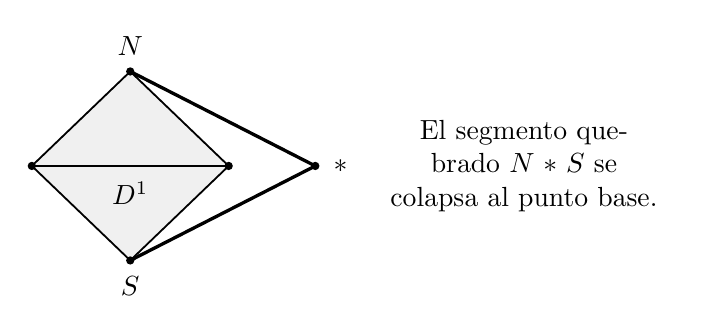
\begin{tikzpicture}[x=1cm,y=1cm,line width=.65pt,line cap=round,line join=round]
\coordinate (N) at (0,1.2);
\coordinate (S) at (0,-1.2);
\coordinate (L) at (-1.25,0);
\coordinate (R) at (1.25,0);
\coordinate (B) at (2.35,0);
\fill[gray!12] (N)--(R)--(S)--(L)--cycle;
\draw (N)--(L)--(S)--(R)--cycle;
\draw (L)--(R);
\draw[very thick] (N)--(B)--(S);
\foreach \p in {N,S,L,R,B}{\fill (\p) circle (1.5pt);}
\node[above=2pt] at (N) {$N$};
\node[below=2pt] at (S) {$S$};
\node[below=2pt] at (0,0) {$D^1$};
\node[right=3pt] at (B) {$*$};
\node[align=center,text width=3.6cm] at (5,0) {El segmento quebrado $N* S$ se colapsa al punto base.};
\end{tikzpicture}
\end{center}
El rombo es un disco $D^2$; puede obtenerse de $D^1\times I$ colapsando cada extremo por separado a $N$ y $S$. El segmento quebrado $N* S$ se colapsa después al punto base, identificando esos vértices. En el pushout podemos usar directamente $D^1\times I\cong D^2$, porque su aplicación de borde ya envía ambos extremos al punto base.

Repitiendo el argumento en las etapas de la construcción celular, y usando que la suspensión preserva también sus colímites, concluimos que $\Sigma X$ es un complejo celular. Su estructura tiene una $(n+1)$-celda por cada $n$-celda de $X$ distinta del punto base. El punto base permanece como una $0$-celda y no genera una celda adicional al suspender.

% P27--P28.
\subsection{Celdas estables}

Sea $X$ un espectro celular. Como $\xi_r\colon\Sigma X_r\hookrightarrow X_{r+1}$ es una inclusión de subcomplejo, cada $m$-celda de $X_r$, distinta del punto base, determina una $(m+1)$-celda de $X_{r+1}$. Queremos considerar estas dos celdas como representantes de una misma celda del espectro.

Para suspender una función característica $\Psi\colon D^d\to X$, la extendemos a una aplicación punteada $\Psi_+\colon D^d_+\to X$. Su suspensión es $\Sigma^n\Psi_+\colon\Sigma^nD^d_+\to\Sigma^nX$. Aquí $\Sigma$ sigue siendo la suspensión reducida y el signo $+$ añade un punto base disjunto. Como en la construcción anterior, una función característica de la celda suspendida se obtiene precomponiendo con $q\colon D^{d+n}\to\Sigma^nD^d_+$; véase \cite[Lema~2.6.1.1]{malkiewich}. Para $n\ge1$, $q$ es el cociente que, en el modelo $D^{d+n}\cong D^d\times I^n$, colapsa $D^d\times\partial I^n$ al punto base. Para $n=0$, es la inclusión $D^d\to D^d_+$. En particular, $\Sigma^nD^d_+$ no se identifica con el disco: ya $\Sigma D^0_+=S^1$.\label{nota:c10-suspension-celda}

Sean ahora $\Phi\colon D^m\to X_r$ y $\Psi\colon D^{m-n}\to X_{r-n}$ funciones características, con $0\le n\le\min\{m,r\}$. La suspensión de la segunda celda está representada por $\Sigma^n\Psi_+\circ q\colon D^m\to\Sigma^nX_{r-n}$. Distinguimos así la aplicación punteada suspendida de la función característica cuyo dominio es un disco.

Diremos que $\Phi$ es la \emph{$n$-ésima suspensión de $\Psi$ en el espectro} si, con funciones características compatibles, conmuta el diagrama
\[
\begin{tikzcd}[column sep=large]
D^m \arrow[r,"q"] \arrow[ddddrr,"\Phi"']
& \Sigma^nD^{m-n}_+ \arrow[r,"\Sigma^n\Psi_+"]
& \Sigma^nX_{r-n}
\arrow[d,"\Sigma^{n-1}\xi_{r-n}"]\\
&& \Sigma^{n-1}X_{r-n+1} \arrow[d]\\
&& \vdots \arrow[d]\\
&& \Sigma X_{r-1} \arrow[d,"\xi_{r-1}"]\\
&& X_r.
\end{tikzcd}
\]
El diagrama se escribe para $n\ge2$; para $n=1$, el compuesto es $\xi_{r-1}\circ\Sigma\Psi_+\circ q$. Si $n=0$, no intervienen morfismos estructurales y $\Psi_+\circ q=\Psi$. La expresión ``suspensión de una celda'' incluye, por tanto, tanto la suspensión como el paso a los niveles siguientes mediante los morfismos estructurales.

\begin{defi}\label{defi:c10-celda-estable}
Una \emph{celda estable} de $X$ es una clase de celdas distintas del punto base bajo la relación de equivalencia generada por identificar cada celda con su suspensión en el nivel siguiente. Si una clase está representada por $\Phi\colon D^m\to X_r$, su \emph{dimensión estable} es $m-r$.
\end{defi}

La dimensión está bien definida: al suspender una vez, tanto la dimensión de la celda como el nivel del espectro aumentan en uno, de modo que $(m+1)-(r+1)=m-r$. En particular, una celda estable puede tener dimensión negativa. La relación se establece entre las celdas de la estructura celular elegida; las funciones características solo sirven para describirla y se escogen de manera compatible con la suspensión.

\subsection{El espectro esfera}

Consideremos $\mathbb S=(S^0,S^1,S^2,\ldots)$ con su estructura celular habitual: en $S^0=\{-1,1\}$ tomamos $1$ como punto base y $-1$ como la otra $0$-celda. Esta última tiene función característica $\Phi\colon D^0\to\mathbb S_0$, con $\Phi(D^0)=\{-1\}$, y representa una celda estable de dimensión $0-0=0$.

Al suspender, el segmento que procede del punto base se colapsa y el segmento procedente de $-1$ da la única $1$-celda no trivial de $S^1$. El siguiente dibujo representa ese paso:
\begin{center}
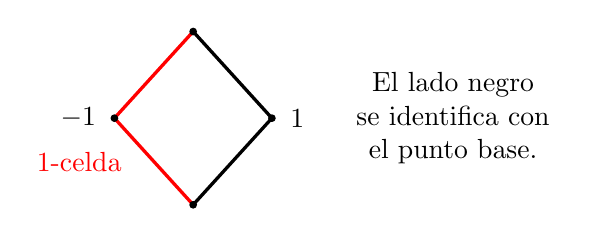
\begin{tikzpicture}[x=1cm,y=1cm,line width=.7pt,line cap=round,line join=round]
\coordinate (N) at (0,1.1);
\coordinate (S) at (0,-1.1);
\coordinate (L) at (-1,0);
\coordinate (R) at (1,0);
\draw[red,very thick] (N)--(L)--(S);
\draw[very thick] (N)--(R)--(S);
\foreach \p in {N,S,L,R}{\fill (\p) circle (1.4pt);}
\node[left=3pt] at (L) {$-1$};
\node[right=3pt] at (R) {$1$};
\node[red,left=8pt] at (-.5,-.55) {$1$-celda};
\node[align=center,text width=3.1cm] at (3.3,0) {El lado negro se identifica con el punto base.};
\end{tikzpicture}
\end{center}
La $1$-celda de $S^1$ es la suspensión de la $0$-celda de $S^0$, y por ello representa la misma celda estable. De igual manera, la única $r$-celda distinta del punto base en $S^r$ es la suspensión iterada de aquella $0$-celda. Todas estas celdas representan una sola clase y tienen dimensión estable $r-r=0$. Con esta estructura, $\mathbb S$ tiene exactamente una $0$-celda estable.

Esta afirmación depende de la estructura celular escogida. Como se aclaró al final de la clase, se pueden elegir otras estructuras celulares compatibles en las esferas, con más celdas; el número de celdas estables no se afirma invariante bajo esos cambios.
